% !TEX program = xelatex
\documentclass[aspectratio=169]{beamer}
\usepackage{amsmath}
\usepackage{amssymb}
\usepackage{graphicx}
\usepackage{tcolorbox}
\usepackage{booktabs}
\usepackage{colortbl}
\usepackage{xcolor}
\usepackage{tikz}
\usetikzlibrary{angles,quotes}
\usepackage[utf8]{inputenc}

% Custom colors
\definecolor{primary}{RGB}{41, 128, 185}
\definecolor{secondary}{RGB}{52, 152, 219}
\definecolor{accent}{RGB}{231, 76, 60}
\definecolor{lightgray}{RGB}{236, 240, 241}

% Theme customization
\usetheme{Madrid}
\usecolortheme{whale}
\setbeamercolor{structure}{fg=primary}
\setbeamercolor{background canvas}{bg=white}
\setbeamercolor{normal text}{fg=black}

% Title page info
\title{Pre-Calculus 11}
\subtitle{Sine Law}
\author{Created by Yi-Chen Lin}
\date{\today}

\begin{document}

% Title Page
\begin{frame}
    \titlepage
\end{frame}

% I) SINE LAW
\begin{frame}{Sine Law}
    \begin{tcolorbox}[colback=lightgray,colframe=primary,title=The Sine Law]
        \footnotesize
        \begin{itemize}
            \item The Sine Law is used for solving triangles that are not right triangles.
            \item Name each side with the letter opposite its angle: $a$ opposite $A$, $b$ opposite $B$, $c$ opposite $C$.
            \item \textbf{Sine Law:}
            \[
                \frac{a}{\sin A} = \frac{b}{\sin B} = \frac{c}{\sin C}
            \]
            \item You can use the Sine Law when you are given one angle and its opposite side.
        \end{itemize}
    \end{tcolorbox}
    
    \vspace{1em}
    \begin{center}
    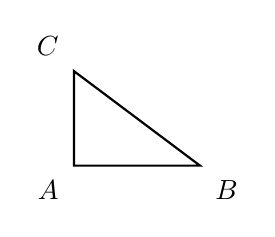
\begin{tikzpicture}[scale=0.4]
    \coordinate (A) at (0,0);
    \coordinate (B) at (4,0);
    \coordinate (C) at (0,3);
    \draw[thick] (A) -- (B) -- (C) -- cycle;
    % Angle labels
    \node[below left=2pt] at (A) {$A$};
    \node[below right=2pt] at (B) {$B$};
    \node[above left=2pt] at (C) {$C$};
    % Side labels
\end{tikzpicture}

    \end{center}
\end{frame}

% Example: Solving for a side using Sine Law
\begin{frame}{Example: Solving for a Side}
    \begin{tcolorbox}[colback=lightgray,colframe=primary,title=Question]
        \footnotesize
        In $\triangle ABC$, $a = 10$ cm, $A = 50^\circ$, $C = 65^\circ$. Solve for side $c$.
    \end{tcolorbox}
\end{frame}

\begin{frame}{Example: Solving for a Side}
    \begin{tcolorbox}[colback=lightgray,colframe=primary,title=Solution]
        \footnotesize
        \begin{columns}
            \column{0.55\textwidth}
            \begin{align*}
                \frac{a}{\sin A} &= \frac{c}{\sin C} \\
                \frac{10}{\sin 50^\circ} &= \frac{c}{\sin 65^\circ} \\
                c &= \frac{10 \cdot \sin 65^\circ}{\sin 50^\circ} \approx 12.36 \text{ cm}
            \end{align*}
            \column{0.45\textwidth}
            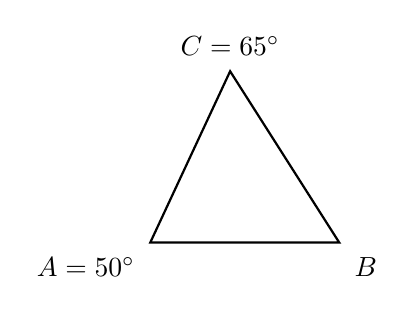
\begin{tikzpicture}[scale=0.6]
                \coordinate (A) at (0,0);
                \coordinate (B) at (4,0);
                \coordinate (C) at ({4*cos(65)},{4*sin(65)});
                \draw[thick] (A) -- (B) -- (C) -- cycle;
                % Angle labels
                \node[below left=2pt] at (A) {$A=50^\circ$};
                \node[below right=2pt] at (B) {$B$};
                \node[above=2pt] at (C) {$C=65^\circ$};
            \end{tikzpicture}
        \end{columns}
    \end{tcolorbox}
\end{frame}

% Practice: Find the value of x
\begin{frame}{Practice: Find the Value of $x$}
    \begin{tcolorbox}[colback=lightgray,colframe=accent,title=Practice]
        \footnotesize
        In $\triangle ABC$, $a = 15$ m, $A = 37^\circ$, $C = 72^\circ$, $c = x$. Find $x$.
    \end{tcolorbox}
\end{frame}

\begin{frame}{Practice: Find the Value of $x$}
    \begin{tcolorbox}[colback=lightgray,colframe=accent,title=Solution]
        \footnotesize
        \begin{columns}
            \column{0.55\textwidth}
            \begin{align*}
                \frac{a}{\sin A} &= \frac{c}{\sin C} \\
                \frac{15}{\sin 37^\circ} &= \frac{x}{\sin 72^\circ} \\
                x &= \frac{15 \cdot \sin 72^\circ}{\sin 37^\circ} \approx 24.18 \text{ m}
            \end{align*}
            \column{0.45\textwidth}
            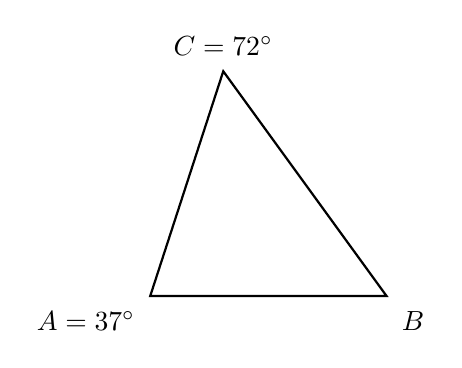
\begin{tikzpicture}[scale=0.6]
                \coordinate (A) at (0,0);
                \coordinate (B) at (5,0);
                \coordinate (C) at ({5*cos(72)},{5*sin(72)});
                \draw[thick] (A) -- (B) -- (C) -- cycle;
                % Angle labels
                \node[below left=2pt] at (A) {$A=37^\circ$};
                \node[below right=2pt] at (B) {$B$};
                \node[above=2pt] at (C) {$C=72^\circ$};
            \end{tikzpicture}
        \end{columns}
    \end{tcolorbox}
\end{frame}

% II) FINDING MISSING ANGLES
\begin{frame}{Finding Missing Angles}
    \begin{tcolorbox}[colback=lightgray,colframe=primary,title=Finding Angles with Sine Law]
        \footnotesize
        \begin{itemize}
            \item To find an angle, use the inverse sine function.
            \item If the angle is obtuse, the answer is in Quadrant II: $\theta = 180^\circ - \sin^{-1}(\text{ratio})$.
        \end{itemize}
    \end{tcolorbox}
\end{frame}

% Example: Solving for an angle
\begin{frame}{Example: Solving for an Angle}
    \begin{tcolorbox}[colback=lightgray,colframe=primary,title=Question]
        \footnotesize
        In $\triangle ABC$, $a = 11$ in, $A = 40^\circ$, $c = 8$ in. Solve for angle $C$.
    \end{tcolorbox}
\end{frame}

\begin{frame}{Example: Solving for an Angle}
    \begin{tcolorbox}[colback=lightgray,colframe=primary,title=Solution]
        \footnotesize
        \begin{columns}
            \column{0.55\textwidth}
            \begin{align*}
                \frac{a}{\sin A} &= \frac{c}{\sin C} \\
                \frac{11}{\sin 40^\circ} &= \frac{8}{\sin C} \\
                \sin C &= \frac{8 \cdot \sin 40^\circ}{11} \approx 0.4646 \\
                C &= \sin^{-1}(0.4646) \approx 27.7^\circ
            \end{align*}
            \column{0.45\textwidth}
            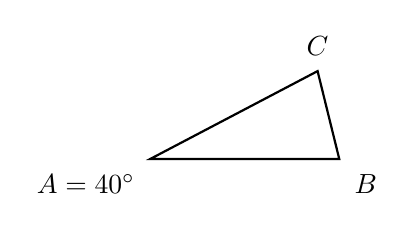
\begin{tikzpicture}[scale=0.6]
                \coordinate (A) at (0,0);
                \coordinate (B) at (4,0);
                \coordinate (C) at ({4*cos(27.7)},{4*sin(27.7)});
                \draw[thick] (A) -- (B) -- (C) -- cycle;
                % Angle labels
                \node[below left=2pt] at (A) {$A=40^\circ$};
                \node[below right=2pt] at (B) {$B$};
                \node[above=2pt] at (C) {$C$};
            \end{tikzpicture}
        \end{columns}
    \end{tcolorbox}
\end{frame}

% Practice: Solve for the missing angle
\begin{frame}{Practice: Solve for the Missing Angle}
    \begin{tcolorbox}[colback=lightgray,colframe=accent,title=Practice]
        \footnotesize
        In $\triangle ABC$, $a = 7.5$, $A = 50^\circ$, $c = 15$. Solve for angle $C$.
    \end{tcolorbox}
\end{frame}

\begin{frame}{Practice: Solve for the Missing Angle}
    \begin{tcolorbox}[colback=lightgray,colframe=accent,title=Solution]
        \footnotesize
        \begin{columns}
            \column{0.55\textwidth}
            \begin{align*}
                \frac{a}{\sin A} &= \frac{c}{\sin C} \\
                \frac{7.5}{\sin 50^\circ} &= \frac{15}{\sin C} \\
                \sin C &= \frac{15 \cdot \sin 50^\circ}{7.5} \approx 1.148 \\
                \text{No solution: } \sin C > 1
            \end{align*}
            \column{0.45\textwidth}
            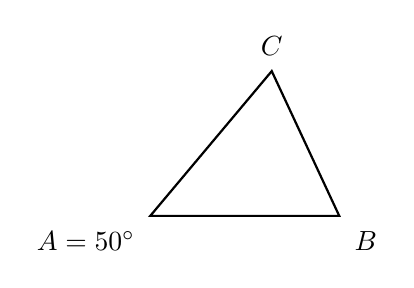
\begin{tikzpicture}[scale=0.6]
                \coordinate (A) at (0,0);
                \coordinate (B) at (4,0);
                \coordinate (C) at ({4*cos(50)},{4*sin(50)});
                \draw[thick] (A) -- (B) -- (C) -- cycle;
                % Angle labels
                \node[below left=2pt] at (A) {$A=50^\circ$};
                \node[below right=2pt] at (B) {$B$};
                \node[above=2pt] at (C) {$C$};
            \end{tikzpicture}
        \end{columns}
    \end{tcolorbox}
\end{frame}

% III) OBTUSE ANGLE CASES
\begin{frame}{Triangles with Obtuse Angles}
    \begin{tcolorbox}[colback=lightgray,colframe=primary,title=Obtuse Angles]
        \footnotesize
        \begin{itemize}
            \item An obtuse angle is greater than $90^\circ$.
            \item In the $xy$-plane, the angle will be in Quadrant II.
            \item If $\sin B = x$ and $B$ is obtuse, $B = 180^\circ - \sin^{-1}(x)$.
        \end{itemize}
    \end{tcolorbox}
\end{frame}

% Example: Obtuse Angle
\begin{frame}{Example: Obtuse Angle}
    \begin{tcolorbox}[colback=lightgray,colframe=primary,title=Question]
        \footnotesize
        In $\triangle ABC$, $a = 13$ m, $b = 18.5$ m, $A = 40^\circ$. Solve for angle $B$.
    \end{tcolorbox}
\end{frame}

\begin{frame}{Example: Obtuse Angle}
    \begin{tcolorbox}[colback=lightgray,colframe=primary,title=Solution]
        \footnotesize
        \begin{columns}
            \column{0.55\textwidth}
            \begin{align*}
                \frac{a}{\sin A} &= \frac{b}{\sin B} \\
                \frac{13}{\sin 40^\circ} &= \frac{18.5}{\sin B} \\
                \sin B &= \frac{18.5 \cdot \sin 40^\circ}{13} \approx 0.914 \\
                B &= 180^\circ - \sin^{-1}(0.914) \approx 114.8^\circ
            \end{align*}
            \column{0.45\textwidth}
            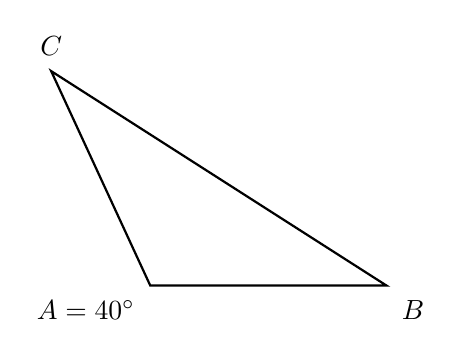
\begin{tikzpicture}[scale=0.6]
                \coordinate (A) at (0,0);
                \coordinate (B) at (5,0);
                \coordinate (C) at ({5*cos(114.8)},{5*sin(114.8)});
                \draw[thick] (A) -- (B) -- (C) -- cycle;
                % Angle labels
                \node[below left=2pt] at (A) {$A=40^\circ$};
                \node[below right=2pt] at (B) {$B$};
                \node[above=2pt] at (C) {$C$};
            \end{tikzpicture}
        \end{columns}
    \end{tcolorbox}
\end{frame}

% Practice: Find the obtuse angle
\begin{frame}{Practice: Find the Obtuse Angle}
    \begin{tcolorbox}[colback=lightgray,colframe=accent,title=Practice]
        \footnotesize
        In $\triangle ABC$, $a = 12$ m, $b = 19$ m, $A = 35^\circ$. Solve for angle $B$ (obtuse).
    \end{tcolorbox}
\end{frame}

\begin{frame}{Practice: Find the Obtuse Angle}
    \begin{tcolorbox}[colback=lightgray,colframe=accent,title=Solution]
        \footnotesize
        \begin{columns}
            \column{0.55\textwidth}
            \begin{align*}
                \frac{a}{\sin A} &= \frac{b}{\sin B} \\
                \frac{12}{\sin 35^\circ} &= \frac{19}{\sin B} \\
                \sin B &= \frac{19 \cdot \sin 35^\circ}{12} \approx 0.908 \\
                B &= 180^\circ - \sin^{-1}(0.908) \approx 114.8^\circ
            \end{align*}
            \column{0.45\textwidth}
            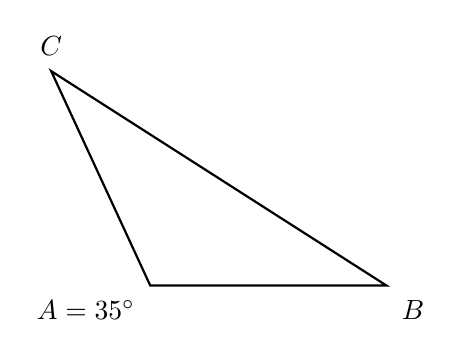
\begin{tikzpicture}[scale=0.6]
                \coordinate (A) at (0,0);
                \coordinate (B) at (5,0);
                \coordinate (C) at ({5*cos(114.8)},{5*sin(114.8)});
                \draw[thick] (A) -- (B) -- (C) -- cycle;
                % Angle labels
                \node[below left=2pt] at (A) {$A=35^\circ$};
                \node[below right=2pt] at (B) {$B$};
                \node[above=2pt] at (C) {$C$};
            \end{tikzpicture}
        \end{columns}
    \end{tcolorbox}
\end{frame}

% IV) SINE LAW PROOF
\begin{frame}{Proof of the Sine Law}
    \begin{tcolorbox}[colback=lightgray,colframe=primary,title=Proof]
        \footnotesize
        \begin{columns}
            \column{0.55\textwidth}
            \begin{itemize}
                \item Draw an altitude from one vertex and use right triangle trigonometry to show:
                \[
                    \frac{a}{\sin A} = \frac{b}{\sin B} = \frac{c}{\sin C}
                \]
            \end{itemize}
            \column{0.45\textwidth}
            \begin{tikzpicture}[scale=0.6]
                \coordinate (A) at (0,0);
                \coordinate (B) at (4,0);
                \coordinate (C) at ({4*cos(70)},{4*sin(70)});
                \draw[thick] (A) -- (B) -- (C) -- cycle;
                \draw[dashed] (B) -- ($(A)!0.7!(C)$);
                % Angle labels
                \node[below left=2pt] at (A) {$A$};
                \node[below right=2pt] at (B) {$B$};
                \node[above=2pt] at (C) {$C$};
            \end{tikzpicture}
        \end{columns}
    \end{tcolorbox}
\end{frame}

\end{document} 